%% Creator: Inkscape inkscape 0.92.3, www.inkscape.org
%% PDF/EPS/PS + LaTeX output extension by Johan Engelen, 2010
%% Accompanies image file 'architecture.pdf' (pdf, eps, ps)
%%
%% To include the image in your LaTeX document, write
%%   \input{<filename>.pdf_tex}
%%  instead of
%%   \includegraphics{<filename>.pdf}
%% To scale the image, write
%%   \def\svgwidth{<desired width>}
%%   \input{<filename>.pdf_tex}
%%  instead of
%%   \includegraphics[width=<desired width>]{<filename>.pdf}
%%
%% Images with a different path to the parent latex file can
%% be accessed with the `import' package (which may need to be
%% installed) using
%%   \usepackage{import}
%% in the preamble, and then including the image with
%%   \import{<path to file>}{<filename>.pdf_tex}
%% Alternatively, one can specify
%%   \graphicspath{{<path to file>/}}
%% 
%% For more information, please see info/svg-inkscape on CTAN:
%%   http://tug.ctan.org/tex-archive/info/svg-inkscape
%%
\begingroup%
  \makeatletter%
  \providecommand\color[2][]{%
    \errmessage{(Inkscape) Color is used for the text in Inkscape, but the package 'color.sty' is not loaded}%
    \renewcommand\color[2][]{}%
  }%
  \providecommand\transparent[1]{%
    \errmessage{(Inkscape) Transparency is used (non-zero) for the text in Inkscape, but the package 'transparent.sty' is not loaded}%
    \renewcommand\transparent[1]{}%
  }%
  \providecommand\rotatebox[2]{#2}%
  \newcommand*\fsize{\dimexpr\f@size pt\relax}%
  \newcommand*\lineheight[1]{\fontsize{\fsize}{#1\fsize}\selectfont}%
  \ifx\svgwidth\undefined%
    \setlength{\unitlength}{557.62309494bp}%
    \ifx\svgscale\undefined%
      \relax%
    \else%
      \setlength{\unitlength}{\unitlength * \real{\svgscale}}%
    \fi%
  \else%
    \setlength{\unitlength}{\svgwidth}%
  \fi%
  \global\let\svgwidth\undefined%
  \global\let\svgscale\undefined%
  \makeatother%
  \begin{picture}(1,0.45467189)%
    \lineheight{1}%
    \setlength\tabcolsep{0pt}%
    \put(0,0){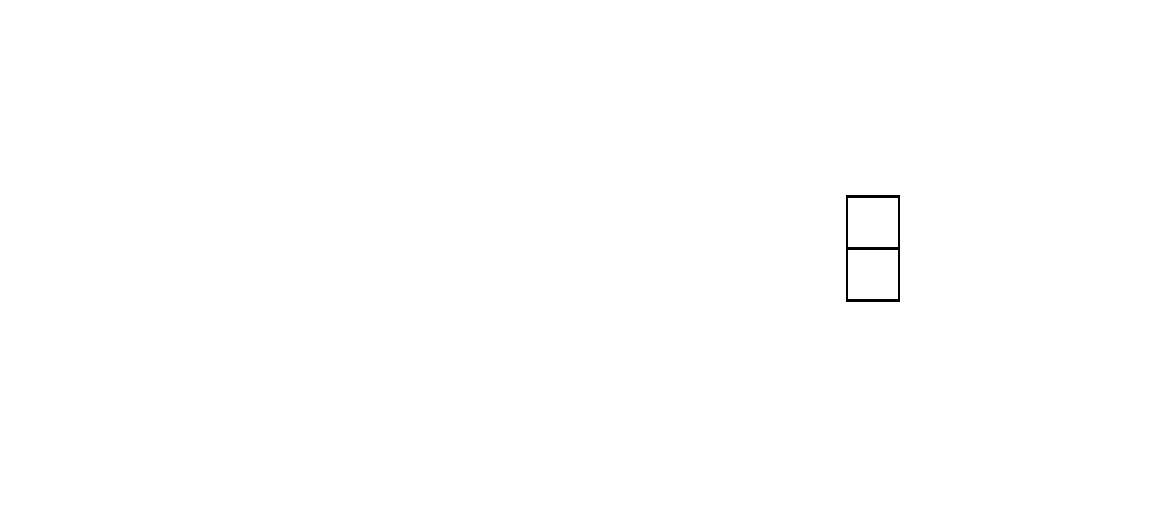
\includegraphics[width=\unitlength,page=1]{architecture.pdf}}%
    \put(0,0){\includegraphics[width=\unitlength,page=2]{architecture.pdf}}%
    \put(0,0){\includegraphics[width=\unitlength,page=4]{architecture.pdf}}%
    \put(0,0){\includegraphics[width=\unitlength,page=5]{architecture.pdf}}%
    \put(0.01531034,0.23278947){\color[rgb]{0,0,0}\makebox(0,0)[lt]{\lineheight{1.25}\smash{\begin{tabular}[t]{l}$x$\end{tabular}}}}%
    \put(0.104763,0.37076041){\color[rgb]{0,0,0}\makebox(0,0)[lt]{\lineheight{1.25}\smash{\begin{tabular}[t]{l}clamp(0,1)\end{tabular}}}}%
    \put(0.104763,0.10174931){\color[rgb]{0,0,0}\makebox(0,0)[lt]{\lineheight{1.25}\smash{\begin{tabular}[t]{l}clamp(0,1)\end{tabular}}}}%
    \put(0,0){\includegraphics[width=\unitlength,page=3]{architecture.pdf}}%
    \put(0.1373542,0.42287233){\color[rgb]{0,0,0}\makebox(0,0)[lt]{\lineheight{1.25}\smash{\begin{tabular}[t]{l}$V_1$\end{tabular}}}}%
    \put(0.1373542,0.04410318){\color[rgb]{0,0,0}\makebox(0,0)[lt]{\lineheight{1.25}\smash{\begin{tabular}[t]{l}$V_2$\end{tabular}}}}%
    \put(0.14084896,0.3056412){\color[rgb]{0,0,0}\makebox(0,0)[lt]{\lineheight{1.25}\smash{\begin{tabular}[t]{l}@\end{tabular}}}}%
    \put(0.14084896,0.15660995){\color[rgb]{0,0,0}\makebox(0,0)[lt]{\lineheight{1.25}\smash{\begin{tabular}[t]{l}@\end{tabular}}}}%
    \put(0,0){\includegraphics[width=\unitlength,page=6]{architecture.pdf}}%
    \put(0.26636246,0.23278947){\color[rgb]{0,0,0}\makebox(0,0)[lt]{\lineheight{1.25}\smash{\begin{tabular}[t]{l}$-$\end{tabular}}}}%
    \put(0,0){\includegraphics[width=\unitlength,page=7]{architecture.pdf}}%
    \put(0.37510308,0.30978841){\color[rgb]{0,0,0}\makebox(0,0)[lt]{\lineheight{1.25}\smash{\begin{tabular}[t]{l}$sign$\end{tabular}}}}%
    \put(0,0){\includegraphics[width=\unitlength,page=8]{architecture.pdf}}%
    \put(0.37510308,0.16112126){\color[rgb]{0,0,0}\makebox(0,0)[lt]{\lineheight{1.25}\smash{\begin{tabular}[t]{l}$zero$\end{tabular}}}}%
    \put(0,0){\includegraphics[width=\unitlength,page=9]{architecture.pdf}}%
    \put(0.51665435,0.303412){\color[rgb]{0,0,0}\makebox(0,0)[lt]{\lineheight{1.25}\smash{\begin{tabular}[t]{l}*\end{tabular}}}}%
    \put(0.51665435,0.15360995){\color[rgb]{0,0,0}\makebox(0,0)[lt]{\lineheight{1.25}\smash{\begin{tabular}[t]{l}*\end{tabular}}}}%
    \put(0,0){\includegraphics[width=\unitlength,page=10]{architecture.pdf}}%
    \put(0.50206793,0.40443271){\color[rgb]{0,0,0}\makebox(0,0)[lt]{\lineheight{1.25}\smash{\begin{tabular}[t]{l}$W^\pm$\end{tabular}}}}%
    \put(0.50206793,0.06146252){\color[rgb]{0,0,0}\makebox(0,0)[lt]{\lineheight{1.25}\smash{\begin{tabular}[t]{l}$W^0$\end{tabular}}}}%
    \put(0,0){\includegraphics[width=\unitlength,page=11]{architecture.pdf}}%
    \put(0,0){\includegraphics[width=\unitlength,page=12]{architecture.pdf}}%
    \put(0.51671497,0.23356021){\color[rgb]{0,0,0}\makebox(0,0)[lt]{\lineheight{1.25}\smash{\begin{tabular}[t]{l}b\end{tabular}}}}%
    \put(0,0){\includegraphics[width=\unitlength,page=13]{architecture.pdf}}%
    \put(0.63950707,0.23396013){\color[rgb]{0,0,0}\makebox(0,0)[lt]{\lineheight{1.25}\smash{\begin{tabular}[t]{l}$+$\end{tabular}}}}%
    \put(0,0){\includegraphics[width=\unitlength,page=14]{architecture.pdf}}%
    \put(0.7389222,0.25628947){\color[rgb]{0,0,0}\makebox(0,0)[lt]{\lineheight{1.25}\smash{\begin{tabular}[t]{l}$z_0$\end{tabular}}}}%
    \put(0.7389222,0.21128947){\color[rgb]{0,0,0}\makebox(0,0)[lt]{\lineheight{1.25}\smash{\begin{tabular}[t]{l}$z_1$\end{tabular}}}}%
    \put(0.89956505,0.25628947){\color[rgb]{0,0,0}\makebox(0,0)[lt]{\lineheight{1.25}\smash{\begin{tabular}[t]{l}$y_0$\end{tabular}}}}%
    \put(0.89956505,0.21128947){\color[rgb]{0,0,0}\makebox(0,0)[lt]{\lineheight{1.25}\smash{\begin{tabular}[t]{l}$y_1$\end{tabular}}}}%
    \put(0.70829551,0.0626421){\color[rgb]{0,0,0}\makebox(0,0)[lt]{\lineheight{1.25}\smash{\begin{tabular}[t]{l}Learnable Parameter\end{tabular}}}}%
    \put(0.65897255,0.0087301){\color[rgb]{0,0,0}\makebox(0,0)[lt]{\lineheight{1.25}\smash{\begin{tabular}[t]{l}@\end{tabular}}}}%
    \put(0.70829551,0.00980301){\color[rgb]{0,0,0}\makebox(0,0)[lt]{\lineheight{1.25}\smash{\begin{tabular}[t]{l}Marix Multiplication\end{tabular}}}}%
    \put(0.82345193,0.27860981){\color[rgb]{0,0,0}\rotatebox{-90}{\makebox(0,0)[lt]{\lineheight{1.25}\smash{\begin{tabular}[t]{l}softmax\end{tabular}}}}}%
    \put(0,0){\includegraphics[width=\unitlength,page=15]{architecture.pdf}}%
  \end{picture}%
\endgroup%
